\chapter{Definição do Ponto de Projeto}
\label{diagramarestricoes}

\section{Diagrama de Restrições}

A partir da definição dos parâmetros da missão típica desejada para a aeronave realizada na primeira parte desta trabalho, dos aeroportos críticos para a operação descritos no \autoref{missao_tipica_parte2} e do MTOW estimado inicial na \autoref{MTOW_inicial} ($20150 kg$), tem-se os requisitos dimensionantes para grupo-motopropulsor e área de asa.
Esses requisitos são representados por meio das curvas de P/W vs W/S para as seguintes condições de acordo com \cite{gudmundsson}:
 
\begin{enumerate}

\item Curva nivelada na velocidade de cruzeiro (95\% MTOW, Altitude de Cruzeiro), $\phi = 30$\textdegree\

\item Distância de decolagem (MTOW, Nível do mar, ISA) de $1200 m$

\item Velocidade de cruzeiro (95\% MTOW, Altitude de Cruzeiro) de 272 KTAS (140 m/s)

\item Teto de serviço (MTOW) de 25000 ft (7600 m)

\item Razão de subida máxima (MTOW, Nível do mar, ISA) de 2200 ft/min (11.2 m/s)

\end{enumerate}

%%%%%%%%%
% ARRUMAR REFERENCIAS
%%%%%%%%%

Os dados necessários para a análise considerando modelo de polar de arrasto simplificado foram baseados em \cite{gudmundsson} para a classe de aeronaves turboélice.
A tabela abaixo resume os valores utilizados para a construção da polar de arrasto simplificada, bem como $C_L$ e $C_D$ na decolagem e $C_{L_{max}}$:

% EQUACAO E TABELA POLAR DE ARRASTO
\begin{equation}
C_D = C_{D_{min}} + k C_L^2
\end{equation}

\begin{table}[H]
\centering
\begin{tabular}{cc}
\toprule
$C_{D_{min}}$ & 0.25 \\
$k$ & 0.30 \\
$C_{L_{TO}}$ & 0.8 \\
$C_{D_{TO}}$  & 0.04 \\
$C_{L_{max}}$ & 2.2 \\
\bottomrule
\end{tabular}
\caption[Dados para polar de arrasto]{Dados para polar de arrasto}
\label{tbl:polar_arrasto}
\end{table}

As curvas resultantes sobrepostas dos requisitos discutidos anteriormente constituem o chamado Diagrama de Restrições.
O objetivo é escolher um ponto ótimo de projeto, ou seja, P/W e W/S para um mínimo P/W e máximo W/S.
Esta é a \textbf{primeira iteração}, que será recalculada conforme estimativas mais precisas de peso e polar de arrasto se tornem possíveis.
Cada restrição escolhida tem seu equacionamento a seguir considerando modelo simplificado da polar de arrasto:

%%%%%%%%%
% DEIXAR EQUAÇÕES BONITAS
%%%%%%%%%


\subsection{Curva nivelada na velocidade de cruzeiro }
\begin{equation}
P/W = q \left[\frac{C_{D_{min}}}{W/S} + \frac{k}{\cos(\phi)q} W/S \right] V_{ref}
\end{equation}

\begin{equation}
q = \frac{1}{2} \rho V_{ref}^2
\end{equation}

\begin{description}
 \item[$V_{ref}$  -]velocidade de cruzeiro
 \item[$S$ -]área de referência da asa
 \item[$\phi$  -]\textit{bank angle}
 \item[$W$  -]MTOW
 \item[$P$  -]Potência Requerida
\end{description}

\subsection{Distância de decolagem}
\begin{equation}
P/W = \left[\frac{V_{LOF}^2}{2 g S_g} + \frac{q C_{D_{TO}}}{W/S} + \mu \left(1 - \frac{q C_{L_{TO}}}{W/S} \right) \right] V_{LOF}
\end{equation}

\begin{equation}
q = \frac{1}{2} \rho \left(\frac{V_{LOF}}{\sqrt{2}} \right)^2
\end{equation}
 
\begin{description}
 \item[$S_g$  -]distância na corrida de decolagem sem contabilizar a distância percorrida até superar o obstáculo exigido por norma, desta forma, $S_g$ representa a pista total disponível para decolagem menos $200 m$ que estima-se ser necessário para conclusão da decolagem. Ou seja, $S_g \leq 1000m$
 \item[$\mu$ -]coeficiente de fricção da pista. $\mu = 0.04$ de acordo com \cite{gudmundsson}.
 \item[$g$  -]aceleração da gravidade
 \item[$V_{LOF}$  -]Velocidade em que a aeronave sai do chão após a corrida, $V_{LOF} = 1.1 V_{ESTOL}$. Nesta condição, o equacionamento foi feito considerando $V_{LOF}/\sqrt{2}$ como uma velocidade média durante a corrida de decolagem.
\end{description}

\subsection{Velocidade de cruzeiro}

\begin{equation}
P/W = \left[ \frac{q C_{D_{min}}}{W/S} + \frac{k W/S}{q} \right] * V_{ref}
\end{equation}

\begin{equation}
q = \frac{1}{2} \rho V_{ref}^2
\end{equation}

\subsection{Teto de serviço}
\begin{equation}
P/W = \left[ \frac{V_V}{V} + \frac{q C_{D_{min}}}{W/S} +  \frac{k W/S}{q} \right] * V 
\end{equation}

\begin{equation}
q = \frac{1}{2} \rho V_{ref}^2
\end{equation}

\begin{equation}
V_V = 100 ft/min 
\end{equation}

\begin{description}
 \item[$V$  -]velocidade para mínima potência requerida 
\end{description}

\subsection{Razão de subida máxima}

\begin{equation}
P/W = \left[ \frac{V_V}{V} + \frac{q C_{D_{min}}}{W/S} +  \frac{k W/S}{q} \right] * V  
\end{equation}

\begin{equation}
q = \frac{1}{2} \rho V^2
\end{equation}

\begin{equation}
V = \sqrt{ \frac{2}{\rho} \frac{W}{S} \sqrt{ \left( \frac{k}{3 C_{D_{min}}}\right)} }
\end{equation}

\section{Espaço de Projeto}

Como as condições de voo modeladas são em diferentes altitudes, a potência requerida foi normalizada para nível do mar de acordo com o método proposto por \cite{anderson1999aircraft}.
O resultado obtido por meio dos requisitos é apresentado abaixo sendo o espaço viável de projeto a região não hachurada.

\begin{figure}[H]
\centering
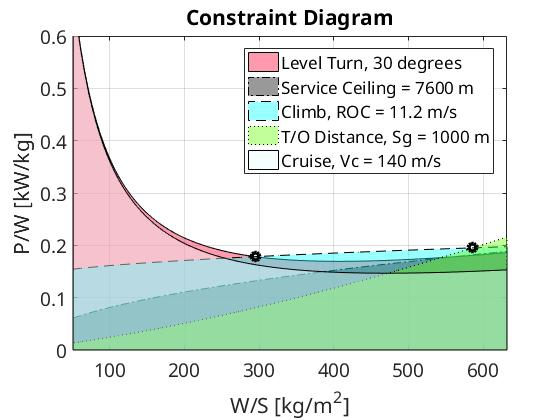
\includegraphics[width=0.75\textwidth]{imagem1.jpg}
\caption[Diagrama de Restrições]{Diagrama de Restrições - Espaço de Projeto}
\label{fig:diagr_restri}
\end{figure}

Os pontos extremos considerados ótimos são os dois pontos destacados no gráfico.
A tabela abaixo apresenta seu valor.

\begin{table}[H]
\centering
\begin{tabular}{ccc}
\toprule
 & P/W & W/S \\ \midrule
(1) & 0.178 kW/kg & 295.6 $kg/m^2$ \\
(2) & 0.195 kW/kg & 586.1 $kg/m^2$ \\
\bottomrule
\end{tabular}
\caption[Pontos Extremos ótimos do Diagrama de Restrições]{Pontos Extremos ótimos do Diagrama de Restrições}
\label{tbl:pontos_extremos}
\end{table}

Deseja-se minimizar a potência requerida atendendo a todos os requisitos imposto.
Além disso, como o objetivo do projeto é minimizar consumo, busca-se o melhor \emph{tradeoff} entre maximizar carga alar e minimizar potência requerida visando desempenho em cruzeiro.
Dessa forma, define-se como pontos de projetos ótimos e viáveis toda a faixa delimitada pelo intervalo dado pelos pontos extremos destacados no gráfico anterior.

Dado a redução do espaço de projeto, o próximo critério a ser avaliado é quanto aos motores comerciais que, dado o MTOW da aeronave definido anteriormente, fornecem a potência requerida dentro do intervalo necessário.
Abaixo tem-se uma tabela com dados de motor da fabricante PW [REF EASA]. 

%%%%%%%%%
% PREENCHER TABELA COM DADOS DA EASA
%%%%%%%%%

\begin{table}[H]
\centering
\begin{tabular}{ccc}
\toprule
Modelo & Potência (MAX) & Potência (T-O) \\ \midrule
PW127 & 2051 kW & 1846 kW \\
PW127B & 2051 kW & 1846 kW \\
PW127D & 2051 kW & 1846 kW \\
PW127E & 1790 kW & 1611 kW \\
PW127F & 2051 kW & 1846 kW \\
PW127G & 2178 kW & 1973 kW \\
PW127M & 2051 kW & 1846 kW \\
PW127M & 2051 kW & 1846 kW \\
\bottomrule
\end{tabular}
\caption[Dados Motores - PW]{Dados Motores PW}
\label{tbl:motores_pw}
\end{table}

Com os dados de motores comerciais e a definição do intervalo de interesse de W/S, tem-se abaixo o gráfico que localiza no espaço de projeto as aeronaves que correspondem a cada motor comercial em termos de W/S e P/S, representados por pontos pretos.

\begin{figure}[H]
\centering
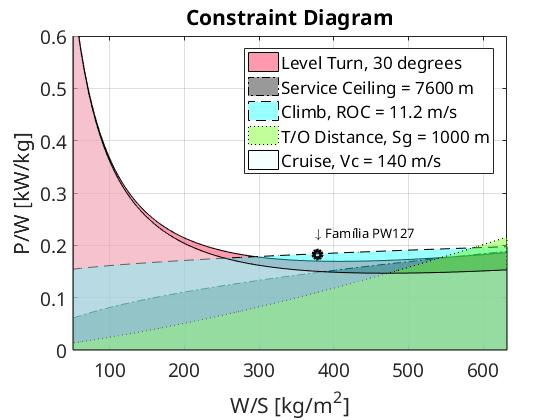
\includegraphics[width=0.75\textwidth]{imagem2.jpg}
\caption[Espaço de Projeto - Motores comerciais]{Espaço de Projeto - Motores comerciais}
\label{fig:diagr_motor}
\end{figure}

\section{Ponto de Projeto - P/W e W/S}
\label{sec:ponto_de_projeto}

Visto que há uma atenção especial para cruzeiro como discutido previamente, define-se como ponto de projeto a aeronave com motor comercial com a máxima carga alar dentro das soluções consideradas ótimas e viáveis.
Abaixo tem-se o modelo de motor, potência típica de decolagem e área alar escolhidos. 

\begin{table}[H]
\centering
\begin{tabular}{ccc}
\toprule
Modelo & Potência (T-O) & S \\ \midrule
PW127 & 1846 kW & $53 m^2$  \\
\bottomrule
\end{tabular}
\caption[Resultado Diagrama de Restrições]{Resultado Diagrama de Restrições}
\label{tbl:resultado_DR}
\end{table}

Sabe-se que a velocidade de estol aumenta com a carga alar.
Por esse motivo, foi verificado qual a velocidade de estol para o ponto de projeto escolhido de forma a garantir que a velocidade de estol não seja alta, o que prejudicaria o desempenho em aproximação e pouso.
Abaixo tem-se o valor calculado para a velocidade de estol considerado seguro para a operação da aeronave.

%%%%%%%%%
% DEIXAR EQUAÇÕES BONITAS
%%%%%%%%%

\begin{equation}
V_{ESTOL} = \sqrt{ \frac
	{W/S}
    {0.5 \cdot \rho \cdot C_{L_{\max}}} 
} = \si{52,5}{m/s} = 102 \si{KEAS}
\end{equation}

A fim de comparar o resultado obtido, decidiu-se representar graficamente no espaço de projeto os concorrentes da aeronave projetada que transportam em torno de 50 passageiros.
A \autoref{tbl:concorrentes_tb} resume os dados dos aviões ATR 42-600 e DASH Q300;
já a \autoref{fig:diagr_concorrentes} apresenta ambas versus o ponto de projeto escolhido. 

\begin{table}[H]
\centering
\begin{tabular}{ccc}
\toprule
 & P/W [\si{kW/kg}] & W/S [\si{kg/m^2}] \\ \midrule
DASH Q300 & 0.167 & 341 \\
ATR 42-600 & 0.174 & 347 \\
Aeronave em projeto & 0.183 & 378 \\
\bottomrule
\end{tabular}
\caption[Comparação - Concorrentes em torno de 50 passageiros]{Comparação - Concorrentes em torno de 50 passageiros}
\label{tbl:concorrentes_tb}
\end{table}

\begin{figure}[H]
\centering
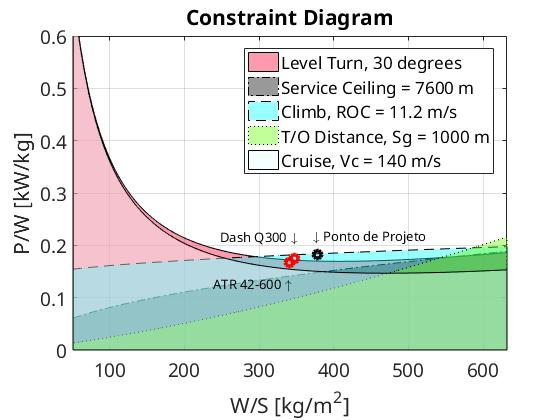
\includegraphics[width=0.75\textwidth]{imagem3.jpg}
\caption[Comparação no espaço de projeto em relação aos concorrentes]{Comparação no espaço de projeto em relação aos concorrentes}
\label{fig:diagr_concorrentes}
\end{figure}

Como pode ser observado, os concorrentes não atendem as restrições impostas a aeronave projetada neste trabalho.
Dessa forma, espera-se que o projeto supere os concorrentes em termos de desempenho para todas as restrições analisadas.
Portanto, conclui-se que a primeira iteração para definição de $S$ e $P$ é promissora e fornece as informações necessárias para os cálculos mais precisos de peso e aerodinâmica, como apresentado nas seções seguintes, bem como o dimensionamento das empenagens.